\chapter{System Analysis and Design}
\label{ch:thiet-ke}

This chapter presents the Evidence Atlas system: what the system must do, how it is organised, which steps a question goes through, and what the system does to ensure that answers are grounded. The content is based on the project's architecture and interface documents \src{14}, \src{23}.

\section{System Requirements}

\subsection{Users and Roles}

The system serves two roles:

\begin{itemize}
    \item \textbf{Buyer.} Asks questions to find books, compare books, see what previous buyers said, and ask about authors and the content of works. Buyers have read-only access to data.
    \item \textbf{Seller.} In addition to the above, sellers can view aggregate statistics by genre, author, publisher and price level, and can try management operations in a simulated environment.
\end{itemize}

Users only choose a role when starting a conversation. Identity, store and the data version in use are all decided by the server based on the access key, not taken from the content the user submits.

\subsection{Functional Requirements}

Table~\ref{tab:yc-chuc-nang} lists the ten main functions the system must provide.

\begin{table}[!htbp]
\caption{Main functional requirements}
\label{tab:yc-chuc-nang}
\cobang
\begin{tabularx}{\linewidth}{C{1.1cm}P{4.2cm}Y}
\toprule
\textbf{No.} & \textbf{Function} & \textbf{Description}\\
\midrule
1 & Search and filter books & Search by title, author, genre; filter by price, rating, page count.\\
2 & Compare and rank & Compare up to 5 books by rating, popularity and price.\\
3 & Summarise reviews & Summarise buyers' praise and complaints based on sampled reviews.\\
4 & Assess reliability & Point out warning signs in reviews (complaints, reviews that are very short or repeated).\\
5 & Market statistics & Aggregate statistics by genre, author, publisher, price range.\\
6 & Questions about works & Answer about the author, themes and original title of a work based on the knowledge base, with citations.\\
7 & Multi-turn conversation & Remember the constraints and books mentioned in previous turns.\\
8 & Propose actions & Prepare actions such as adding to cart or creating an order in a simulated environment; execute only after user confirmation.\\
9 & Progress tracking & Show the steps the system is performing and allow cancellation midway.\\
10 & Refusal with reasons & When evidence is insufficient, state clearly what is missing or ask for clarification instead of guessing.\\
\bottomrule
\end{tabularx}
\end{table}

\subsection{Non-functional Requirements}

\begin{itemize}
    \item \textbf{Grounded.} Every claim about a work must point to a specific source passage. Figures on price, rating and page count must be taken verbatim from the catalogue, never written by the model itself.
    \item \textbf{Bounded.} Each turn has explicit limits on the number of steps, retrievals, waiting time and cost.
    \item \textbf{Secure.} Every request must be authenticated. Permissions are checked on the server, not by hiding buttons in the interface. Error messages do not reveal internal content.
    \item \textbf{Durable.} Conversations, turns and results are stored in the database. Lost connections or resent requests neither lose data nor create duplicate records.
    \item \textbf{Reproducible.} Data, knowledge base and model configuration are all versioned. An experiment can be rerun with exactly the components that were used.
    \item \textbf{Usable.} The interface and messages are in Vietnamese; it is keyboard-accessible; loading, partial success, error and offline states are clearly displayed.
\end{itemize}

\subsection{What the System Does Not Do}

To avoid misunderstanding, the team states explicitly what lies outside the scope:

\begin{itemize}
    \item it does not perform real transactions; all buying and selling operations take place only in a simulated environment;
    \item it does not assert that a review is fake or that a seller is fraudulent, it only points out warning signs;
    \item it makes no claims about trends over time or the current situation, since the data is a past snapshot without timestamps;
    \item it does not guarantee complete elimination of false information; the automatic verification step has errors.
\end{itemize}

\section{Design Principles}

The following four principles govern the design decisions in this chapter.

\textbf{First, the program decides, the model proposes.} Language models are good at understanding questions and writing answers, but they can be wrong without warning. Therefore everything related to permissions, limits, figures and source attribution is handled by conventional program code. The model may only choose among the options the program allows.

\textbf{Second, evidence first, presentation second.} Answers are built from collected facts and source passages, not from the model's memory. No evidence, no claim.

\textbf{Third, explicit limits.} The number of specialists is fixed. The number of steps in a turn is capped. The system does not let agents converse freely with each other, because that approach makes cost hard to control and failures hard to diagnose.

\textbf{Fourth, honesty when things go wrong.} When part of the work fails, the system states clearly which parts succeeded and which did not, instead of silently returning an answer that looks complete.

\section{Overall Architecture}

The system is built as a single application divided into functional modules, running in one process. The team did not split it into multiple microservices, because the project scale does not require it and this approach is simpler to deploy and test. Figure~\ref{fig:kien-truc} shows the layers of the system.

\hinh{kien-truc}{Overall architecture of Evidence Atlas}{fig:kien-truc}

\textbf{Web interface.} The web page where users chat with the assistant. The interface is served by the system's own server, so no separate configuration for cross-origin calls is needed.

\textbf{Gateway.} Every request passes through here. The gateway authenticates the access key, determines who the user is and what permissions they have, limits the number of requests per user within a time window, and attaches a trace identifier to each request for lookup when problems occur.

\textbf{Orchestration core.} The central part, with three jobs: planning within the allowed limits, executing the steps in sequence, and composing and then verifying the answer.

\textbf{Four fixed specialists.} Each specialist is responsible for one type of task and may only use the tools within its own scope (Section~\ref{sec:chuyen-gia}).

\textbf{Database.} A PostgreSQL database stores everything: the book catalogue and reviews, the knowledge base, conversations, turns, and the cost ledger. Specialists may only \emph{read} data, and every read goes through a tool gateway with permission checks.

\textbf{Language model.} An external service. The system sends requests to the model at certain steps and always requires the model to respond in a structured format so that the program can check it.

\section{How a Question Is Processed}
\label{sec:vong-doi}

Figure~\ref{fig:vong-doi} describes the nine steps a turn goes through. White boxes are steps decided entirely by the program; grey boxes are steps in which the language model participates.

\hinh{vong-doi-luot-hoi}{The nine steps of processing a turn}{fig:vong-doi}

\textbf{Step 1 -- Intake.} The system authenticates the sender, checks permissions and records the turn in the database before doing anything else. A request contains only three items: which conversation, a turn identifier generated on the client side, and the question text (at most 2,000 characters).

\textbf{Step 2 -- Version pinning.} The system records the catalogue version and knowledge base version to be used for this turn. If no knowledge base has been published, or the retrieval model does not match the knowledge base, the system refuses to serve rather than run with uncertain data.

\textbf{Step 3 -- Understanding the question.} The program recognises specific information in the question: book titles, price, minimum rating, page count. This uses rules, not the model, so that the numbers in the question are not misinterpreted.

\textbf{Step 4 -- Planning.} The model reads the question and proposes a list of steps, each step being a task assigned to one specialist. The model may only choose from the list of tasks the program allows.

\textbf{Step 5 -- Plan validation.} The program checks the plan: whether the user is allowed to perform each task, whether the steps respect dependency order, and whether the total number of steps exceeds the limit. Invalid plans are rejected.

\textbf{Step 6 -- Execution.} The steps are run in sequence. Each specialist returns two kinds of results: \emph{facts} (e.g.\ the price of a book) and \emph{evidence} (e.g.\ a passage from the knowledge base).

\textbf{Step 7 -- Answer composition.} The model receives the list of facts and evidence, selects the relevant parts, and writes the explanatory text. Figures from the catalogue are inserted verbatim by the program; the model may not rewrite them.

\textbf{Step 8 -- Verification.} Each claim in the draft is checked against its source passage (Section~\ref{sec:kiem-chung}).

\textbf{Step 9 -- Returning the result.} The user receives one of three kinds of response: an answer with sources; a clarifying question; or a refusal stating the reason.

While waiting, the interface receives progress messages (which step is running) and parts of the answer as soon as they are available. Each turn ends with exactly one final message. If the connection drops midway, the interface can query the server for the status and result of that turn.

\section{The Four Specialists}
\label{sec:chuyen-gia}

\subsection{Division of Work}

The system has exactly four specialists, none added or removed at run time. Table~\ref{tab:chuyen-gia} gives the tasks of each specialist and its corresponding limits.

\begin{table}[!htbp]
\caption{The four specialists: tasks and limits}
\label{tab:chuyen-gia}
\cobang
\begin{tabularx}{\linewidth}{P{2.4cm}YY}
\toprule
\textbf{Specialist} & \textbf{Does} & \textbf{Does not}\\
\midrule
Product & Searches, filters, compares and ranks books based on catalogue information. & Does not comment on the content of works.\\
Review & Samples buyer reviews; summarises praise and complaints by aspect; compares reviews across books. & Does not treat the review sample as representative of all buyers.\\
Reliability & Points out warning signs: complaint rate, reviews that are very short or repeated. & Does not assert fake reviews, counterfeit goods or fraud.\\
Market & Computes aggregate statistics by genre, author, publisher, price range, rating level. & Does not discuss trends over time or the current situation.\\
\bottomrule
\end{tabularx}
\end{table}

Knowledge base retrieval does not belong to any single specialist. It is a shared capability, invoked when the question concerns the work itself.

\subsection{Coordination}

Figure~\ref{fig:phoi-hop} shows how the components work together.

\hinh{phoi-hop-chuyen-gia}{The orchestrator assigns tasks to the four specialists and gathers the results}{fig:phoi-hop}

This form of coordination has three characteristics that differ from many multi-agent systems described in the literature:

\begin{itemize}
    \item \textbf{Specialists do not talk to each other.} A specialist only receives tasks from the orchestrator and returns results to it. There is no negotiation or debate between specialists.
    \item \textbf{Specialists have no memory of their own.} All information that must be remembered resides in the orchestrator and the database.
    \item \textbf{Steps run in sequence.} A later step can use the results of an earlier one. For example, for a comparison question, the product specialist first selects up to 5 books; the review specialist compares the reviews of exactly those books; then the reliability specialist examines their reviews.
\end{itemize}

When a step fails, handling depends on the role of that step. If the product specialist finds no book, the later steps have nothing to work on and the system reports that nothing was found. If an auxiliary step fails (e.g.\ reviews cannot be retrieved), the system still answers with what it has and attaches a warning about the missing part.

\subsection{Ranking Formula}

When users ask for suggestions, the product specialist ranks books with a fixed formula rather than letting the model choose by intuition:

\[
\text{Ranking score} = 0.45 \times \frac{r}{5} \;+\; 0.35 \times \frac{\log(1+p)}{\log(1+p_{\max})} \;+\; 0.20 \times \left(1 - \frac{g}{g_{\max}}\right)
\]

Here $r$ is the average rating (on a 5-point scale), $p$ is popularity, $g$ is the selling price; $p_{\max}$ and $g_{\max}$ are the maximum values within the group of books under consideration. Rating has the largest weight (45\%), followed by popularity (35\%) and price (20\%, the lower the price the higher the score). Popularity is log-transformed so that a few best-sellers do not dominate the entire result.

Using a fixed formula has two benefits: the same question always yields the same order, and the system can explain why one book ranks above another. As noted in Chapter~\ref{ch:du-lieu}, popularity is a figure provided by the source and has not been verified as actual sales.

\section{Bounded Planning}

\subsection{Division of Work between Program and Model}

Table~\ref{tab:phan-chia} summarises who does what. This is the most important design decision of the system.

\begin{table}[!htbp]
\caption{Division of work between the program and the language model}
\label{tab:phan-chia}
\cobang
\begin{tabularx}{\linewidth}{YY}
\toprule
\textbf{The program decides} & \textbf{The model may}\\
\midrule
Recognising book titles, prices and ratings in the question & Propose the steps to take, chosen from an allowed list\\
What the user is permitted to do & Choose which facts and evidence are relevant to the question\\
The dependency order between steps & Write the explanatory text in natural language\\
The content of catalogue facts (price, rating, page count) & Revise the draft once when returned by the verification step\\
Ranking scores and the status of each step & \\
Linking claims to source passages and numbering citations & \\
\bottomrule
\end{tabularx}
\end{table}

\subsection{Limits}

Each turn is subject to the limits in Table~\ref{tab:han-muc}. The limits keep the cost and time of a turn always capped, even when the model proposes an overly long plan.

\begin{table}[!htbp]
\caption{Limits applied to a turn}
\label{tab:han-muc}
\cobang
\begin{tabularx}{\linewidth}{YR{4.2cm}}
\toprule
\textbf{Limit} & \textbf{Value}\\
\midrule
Question length & at most 2,000 characters\\
Steps assigned to specialists & at most 8\\
Plan revisions & at most 1\\
Additional read steps when revising the plan & at most 2\\
Books included in comparison or ranking & at most 5\\
Knowledge base retrievals & at most 2\\
Queries per retrieval & at most 4\\
Retrieved text passed to the model & at most 6,000 tokens\\
Draft revisions by the model & at most 1\\
Intermediate results retained & at most 16\\
\bottomrule
\end{tabularx}
\end{table}

\subsection{Fixed Plans and Adaptive Plans}

The system supports two ways of planning, and this is also one of the factors compared in the experiments:

\begin{itemize}
    \item \textbf{Fixed plan.} The program builds the plan itself using predefined rules based on the question type, without consulting the model. The plan is kept unchanged until completion.
    \item \textbf{Adaptive plan.} The model proposes the plan. After initial results are available, the system is allowed to extend the plan exactly once, for example adding a retrieval step when information is found to be missing.
\end{itemize}

Adaptive planning is more flexible but costs additional model calls. Whether that flexibility is worth it is a question answered with data in Chapter~\ref{ch:ket-qua}.

\section{Answer Verification}
\label{sec:kiem-chung}

This is the system's main mechanism against hallucination. Figure~\ref{fig:kiem-chung} describes the process.

\hinh{kiem-chung}{The process of verifying each claim before answering}{fig:kiem-chung}

The draft written by the model is not sent directly to the user. The draft is split into individual claims, and for each claim the model must point to the supporting source passage. Two checks then follow:

\begin{itemize}
    \item \textbf{Check 1 -- does the source passage exist?} The program checks that the quoted passage is indeed in the document, in the pinned version, at the stated position. This check is exact matching, without the model, so it cannot be ``persuaded''. It blocks cases where the model fabricates a citation.
    \item \textbf{Check 2 -- does the source passage say that?} A genuine citation may still be unrelated to the claim. This check examines whether the content of the source passage actually entails the claim.
\end{itemize}

Claims that pass both checks are kept and assigned a citation number. Claims that fail are returned to the model for revision, but \emph{only once}. If they still fail, the claim is dropped from the answer, or the system states clearly that there is insufficient evidence.

The one-revision limit is deliberate. Allowing multiple revisions increases cost and lets the model ``try until it slips through''. One revision is enough to fix wording errors, while claims that are genuinely unsupported should be removed.

The limits of this mechanism must be stated clearly. Check 2 is an automatic check and has errors; it may let a false claim through or wrongly reject a true one. The team therefore does not claim that the system completely eliminates false information, only that every retained claim points to a real source passage so that readers can check it themselves.

\section{State Persistence and Durability}

\subsection{States of a Turn}

Each turn is stored in the database together with its state. Figure~\ref{fig:trang-thai} shows the possible states.

\hinh{trang-thai-luot}{The states of a turn}{fig:trang-thai}

A turn starts in the \emph{pending} state, moves to \emph{running}, and then ends in one of four states: \emph{completed}, \emph{failed}, \emph{cancelled} (the user pressed cancel) or \emph{interrupted} (the server stopped midway).

\subsection{Resending Does Not Create Duplicate Records}

In practice, the network can be unstable and the interface may resend a request. To make resending safe, each turn carries an identifier generated on the client side. When the server receives a request with an identifier it has already seen, it does not rerun the turn but returns the stored status or result. If the resent request does not match the stored turn, the server reports a conflict instead of silently overwriting.

The same principle applies to action confirmation: a confirmation request must carry its own identifier, so pressing confirm twice performs the action only once.

\subsection{Only One Worker Processes a Turn}

When several processes serve requests, it must be ensured that a turn is not processed by two processes in parallel. The system uses the database itself for this: the process that takes on a turn writes its name and a lease expiry into the turn's record; other processes that see the record already owned skip it. If a process hangs beyond the lease, another process may take over; late results from the old process are rejected.

\section{Conversation Memory}

The system has three memory layers with different purposes:

\begin{itemize}
    \item \textbf{Conversation history.} All questions and answers are stored durably so that users can review them.
    \item \textbf{Context passed to the model.} Only part of the history is included in each turn: at most the 8 most recent completed turns, at most 16 stated constraints (e.g.\ ``under VND 150,000''), and at most 8 previously mentioned books. This limit keeps the cost per turn from growing with conversation length.
    \item \textbf{User-declared preferences.} Users can save at most 4 preference entries. The system only remembers what users actively save, and users can view, edit or delete them at any time.
\end{itemize}

The system does not infer preferences from conversation content on its own. This choice makes the assistant slightly less ``smart'', but users always know what the system remembers about them.

\section{Security and Authorisation}

\subsection{Authentication and Permissions}

Every request must carry an access key. The server matches the key against a preconfigured list of users, from which it knows which store the user belongs to and what permissions they have. Users not on the list are rejected. In the browser, the key is held only in the page's temporary memory and is lost when the page is closed; it is not stored on the browser's disk.

Permissions are checked at three layers: at the gateway (whether this person may call this function), at the plan validation step (whether any step in the plan exceeds the user's permissions), and at the tool gateway (whether this data read is permitted). Each resource such as a conversation, turn or action proposal is bound to its owner; others cannot read it.

\subsection{Actions Requiring Confirmation}

The assistant never performs on its own any action that changes data. For requests such as adding to cart or creating an order, the system only prepares a \emph{proposal} and waits. The user reviews the proposal and chooses to confirm or reject it. If, while composing, the model changes the list of books relative to the list approved by the program, the proposal is discarded.

All such actions take place in a simulated environment. There are no real orders and no real payments.

\subsection{Reducing Risks of Using an External Model}

\begin{itemize}
    \item User input and review content are treated as data, not commands. A review containing a sentence like ``ignore previous instructions'' does not change the system's behaviour, because permissions and plans are controlled by the program.
    \item The model must always respond in a structured format. Responses that do not conform are rejected.
    \item The system requires the model provider not to retain the content of requests.
    \item Trace logs are truncated and sensitive parts are masked. Error messages sent to users contain no internal instructions, intermediate data or login information.
    \item Data from the server is displayed by the interface as plain text and is never executed as code.
\end{itemize}

\section{Cost and Failure Control}

Calling a language model costs money and can be slow or fail. The system has the following mechanisms:

\begin{itemize}
    \item \textbf{Cost ledger.} Every model call records its token count and estimated cost in the database. Thanks to this ledger, all cost figures in Chapter~\ref{ch:ket-qua} are measurements, not estimates.
    \item \textbf{Budget cap.} When the total cost reaches the configured cap, the system stops calling the model.
    \item \textbf{Timeout and retry limits.} Each call has a maximum waiting time; calls exceeding it are cancelled.
    \item \textbf{Circuit breaker.} When the model service fails repeatedly, the system pauses calls for a period of time instead of continuing to send requests that are certain to fail.
    \item \textbf{Model usage modes.} The operator can choose one of four modes: model off (rules only), shadow mode (the model runs but its results are not used), hybrid (use the model, fall back to rules on error), and required (report an error if the model fails).
\end{itemize}

\section{System Interface}

The web interface and other programs work with the system through a set of functions listed in Table~\ref{tab:giao-tiep}.

\begin{table}[!htbp]
\caption{Function groups the system exposes externally}
\label{tab:giao-tiep}
\cobang
\begin{tabularx}{\linewidth}{P{3.4cm}Y}
\toprule
\textbf{Group} & \textbf{Functions}\\
\midrule
Identity & Tells who the current user is and which roles they may use.\\
Conversations & Create a new conversation; list one's own conversations; reread a conversation; delete a conversation.\\
Question answering & Send a question and receive the answer at once; or send a question and receive progress along with the answer in parts.\\
Turns & Read the status and result of a turn; cancel a running turn.\\
Action proposals & Read the content of a proposal; confirm; reject.\\
Preferences & Read, save and delete self-declared preferences.\\
Operations & Check whether the system is alive and ready; view operational metrics. Functions for viewing detailed logs require a separate key reserved for operators.\\
\bottomrule
\end{tabularx}
\end{table}

Every response includes the request's trace identifier. When a user reports an error, this identifier alone is enough for the operator to find the entire corresponding processing history.

\section{Technologies Used}

Table~\ref{tab:cong-nghe} lists the main technologies and the reason for choosing each.

\begin{table}[!htbp]
\caption{Main technologies}
\label{tab:cong-nghe}
\cobang
\begin{tabularx}{\linewidth}{P{3.6cm}P{4.6cm}Y}
\toprule
\textbf{Component} & \textbf{Technology} & \textbf{Reason for choice}\\
\midrule
Server & Python, FastAPI & Good support for asynchronous processing and streaming partial results.\\
Database & PostgreSQL & Stores both conventional data and search vectors in one place; supports transactions.\\
Interface & React, TypeScript, Vite & Widely used; type checking helps reduce errors.\\
Interface styling & Tailwind CSS, shadcn/ui & Ready-made components with keyboard and screen reader support.\\
Answer generation model & gpt-5.4-mini (snapshot of 17 March 2026) & Low cost, adequate for the task; pinned to exactly one snapshot so results are reproducible.\\
Semantic search model & text-embedding-3-small & 1,536-dimensional vectors, low cost.\\
Judge model & gpt-6-luna & Different from the answer generation model, to reduce bias in grading.\\
Testing & pytest; type and code-style checkers & Run automatically before every change.\\
\bottomrule
\end{tabularx}
\end{table}

\section{User Interface}

The interface is a web page with three areas (Figure~\ref{fig:giao-dien}; the screenshot is rotated to fit the page and uses illustrative data from the interface test build, not experimental results):

\begin{itemize}
    \item \textbf{Left area -- agents.} Lists the orchestrator and the specialists participating in the current turn, with the status of each component.
    \item \textbf{Centre area -- conversation.} Where the user chooses a role, enters questions and reads answers. Each claim has its citation number placed right next to it. Action proposals appear as separate cards with review and confirm buttons.
    \item \textbf{Right area -- execution details.} Shows the executed plan, usage, the list of evidence sources corresponding to the citation numbers, and the trace identifiers.
\end{itemize}

This layout serves the ``evidence first'' principle: users see not only the answer but also where it comes from and which steps the system took. The interface reflows into a single column on phones.

\begin{figure}[p]
    \centering
    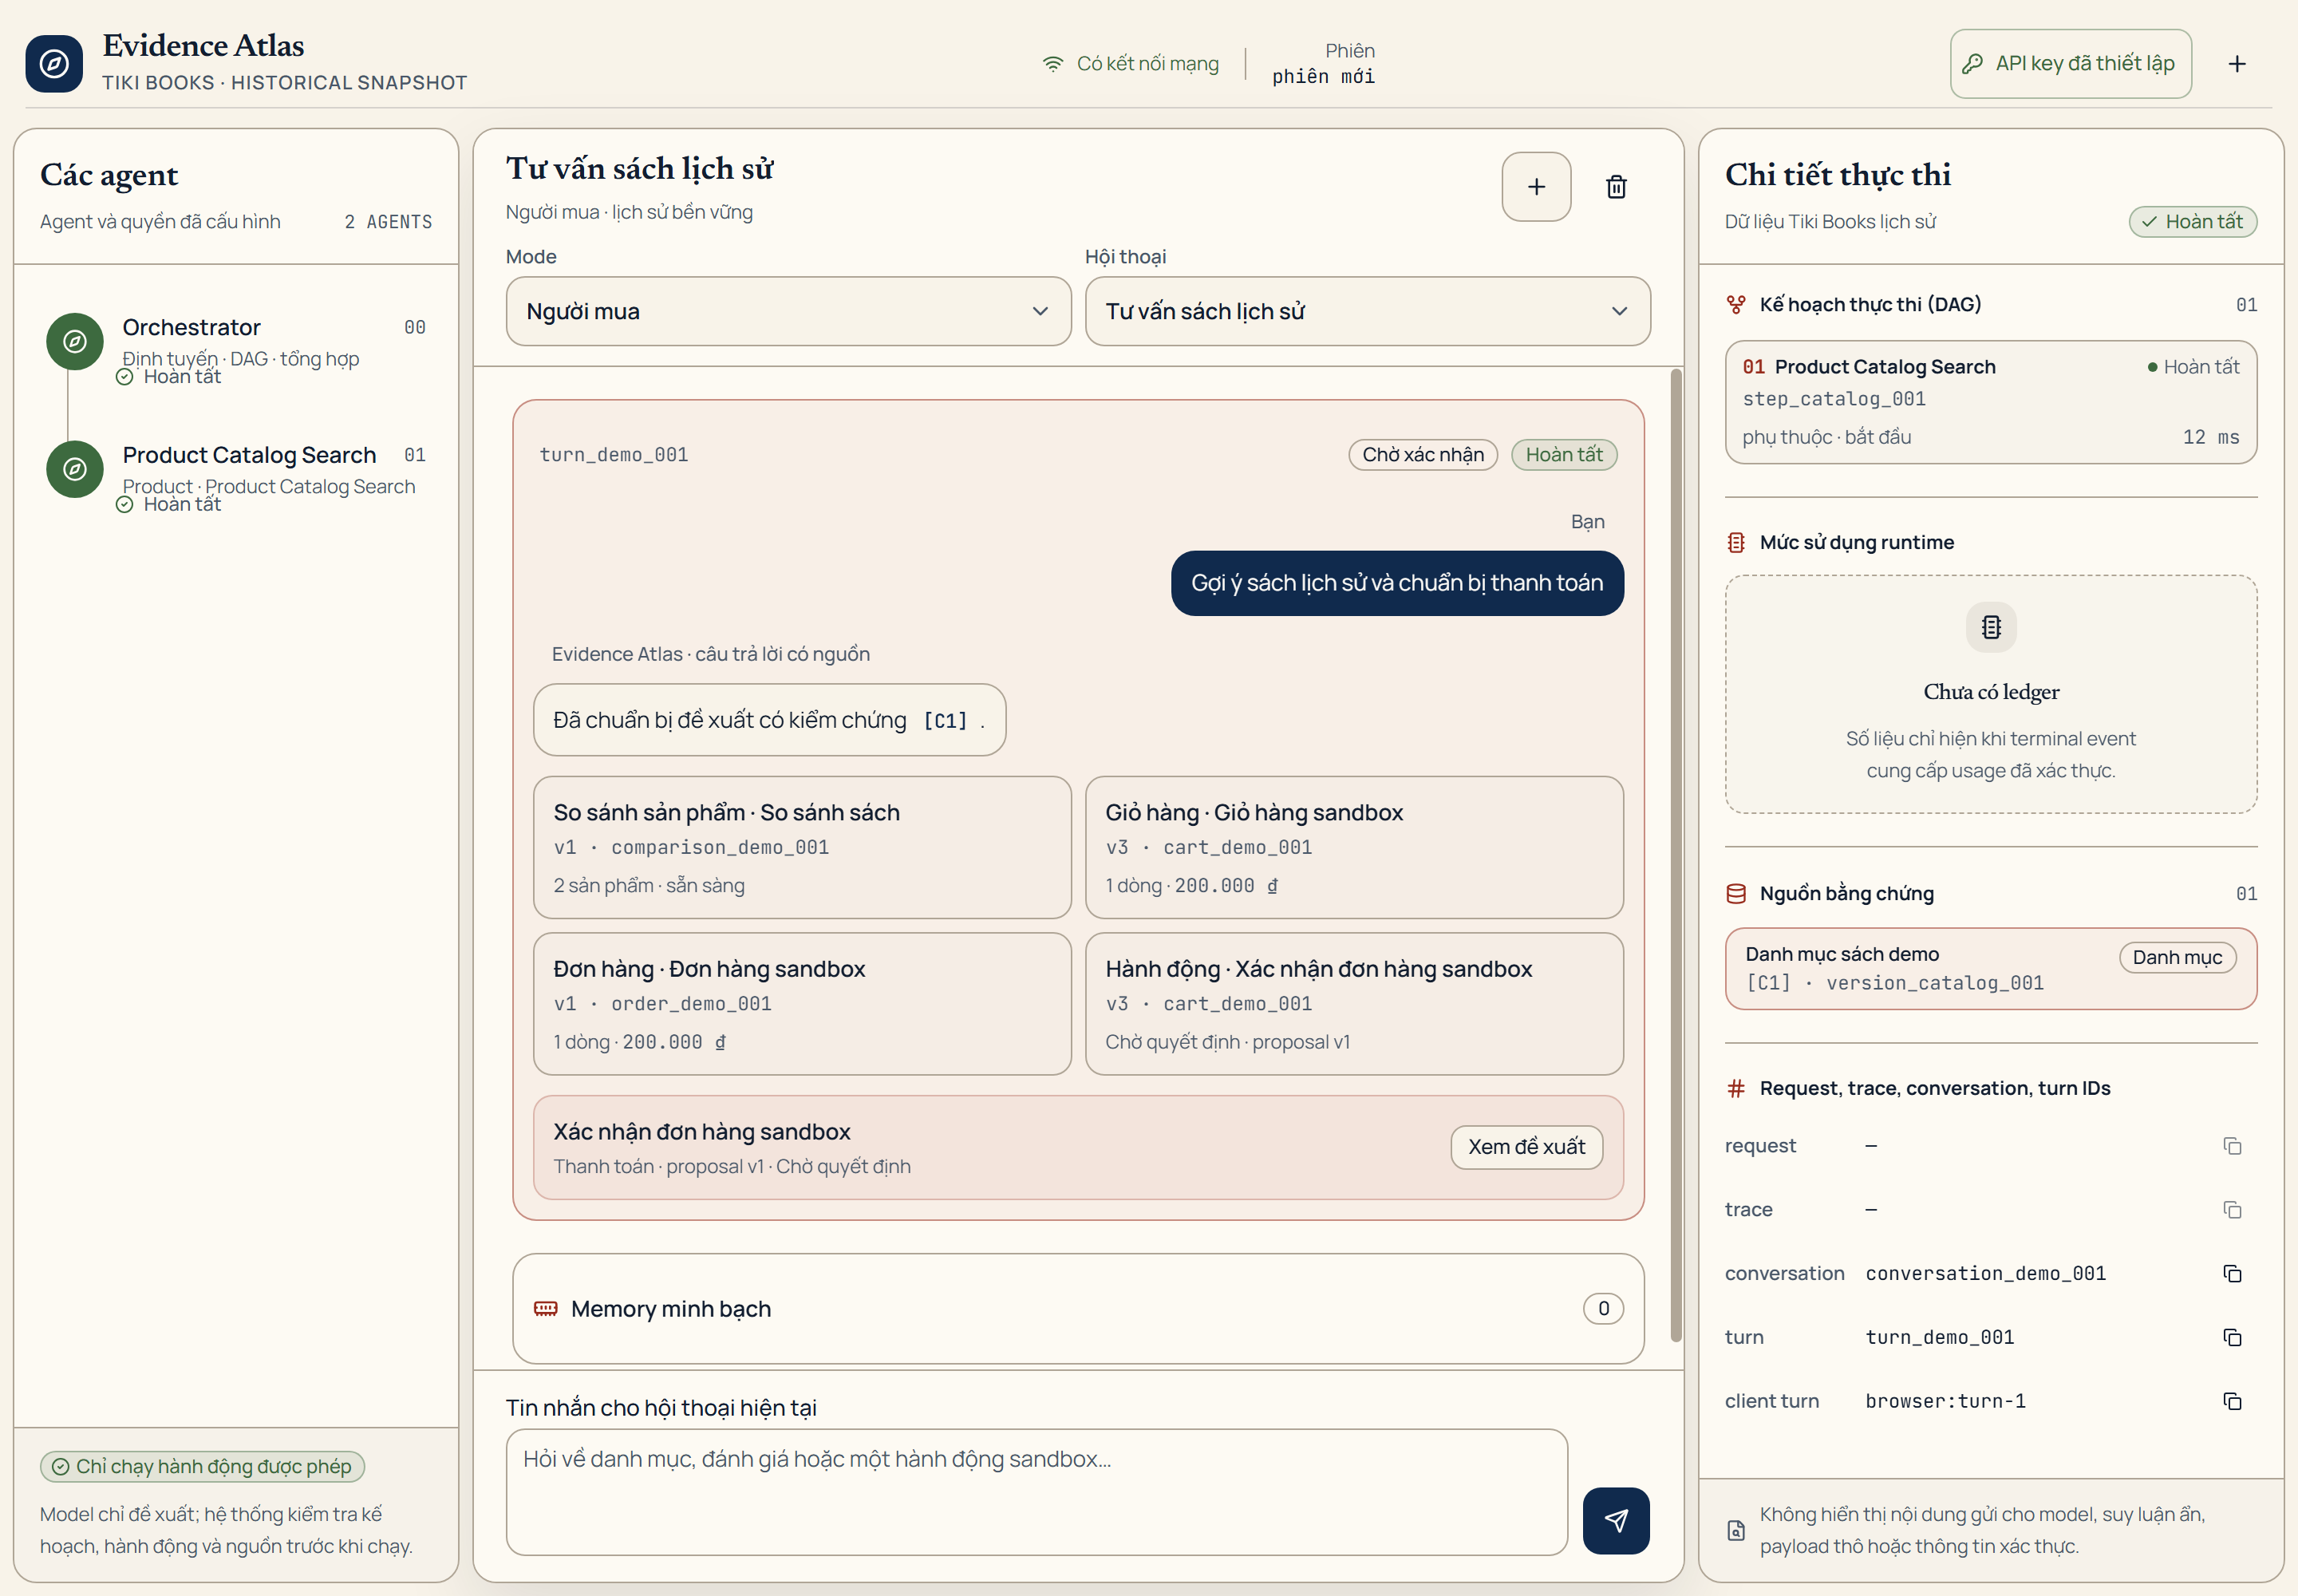
\includegraphics[angle=90,width=0.93\linewidth]{images/giao-dien.png}
    \caption{The Evidence Atlas interface (screenshot with illustrative data; interface text is in Vietnamese)}
    \label{fig:giao-dien}
\end{figure}

\section{Chapter Summary}

Evidence Atlas is a single application consisting of a gateway, an orchestration core, four fixed specialists and a database. A turn goes through nine steps, in which the language model participates in only three: proposing the plan, writing the explanation and assisting verification. All decisions on permissions, limits, figures and citations are held by the program. Answers must pass two checks before reaching the user, and the system chooses to say ``insufficient evidence'' rather than guess. The next chapter presents how the team evaluates this design.
